\section{Exploring the RDD}

The previous section showed that the \rdd can be conceptualized as a
two-step procedure: we first calculate where the replicator dynamic
would take us, then apply diffusion. Since the latter step is the
novel addition, we should look at diffusion in isolation to understand
what the \rdd does. This is what we will do in
Section~\ref{sec:iterated-diffusion}. Section~\ref{sec:simulations}
 then explores how diffusion and fitness-based selection interact.

\subsection{(Iterated) Diffusion}
\label{sec:iterated-diffusion}



Confusion of states should intuitively be a function of their
perceptual similarity. Here and in the following, we assume that the
state space of the sim-max game consists of $n \ge 2$ states that are
equally spaced across the unit interval, including $0$ and $1$. We
assume here that the distance $\card{\mystate{i} - \mystate{j}}$ is
the objective, physical similarity between two states $\mystate{i}$
and $\mystate{j}$. Distance in physical space feeds into a perceptual
similarity function, as described by
\citet{Nosofsky1986:Attention-Simil}:
\begin{align}
  \label{eq:NosofskySim}
  \similarity(\mystate{i}, \mystate{j} \myts ; \myts \impairment) =
      \begin{cases}
    1 & \textrm{if } \impairment = 0 \textrm{ and } \mystate{i} = \mystate{j} \\
    0 & \textrm{if } \impairment = 0 \textrm{ and } \mystate{i} \neq \mystate{j} \\
 \expo \left ( -  \frac{\card{\mystate{i} - \mystate{j}}^s}{ \impairment^2} \right ) \,,& \textrm{otherwise} \\
    \end{cases}
\end{align}
where $\impairment >= 0$ is an imprecision or indiscriminability
parameter. When $\impairment=0$ agents perfectly discriminate between
states; when $\impairment \rightarrow \infty$ agents cannot
discriminate states at all. Figure~\ref{fig:NosofskySim} gives an
impression of Nosofsky-similarity for different parameter
values. Other formalizations of perceptual similarity are possible,
including ones that allow for different discriminability in different
areas of the state space, but we stick with Nosofsky's similarity
function for the time being, because it is a mathematically simple,
yet established notion in mathematical psychology.

\begin{figure}
  \centering

  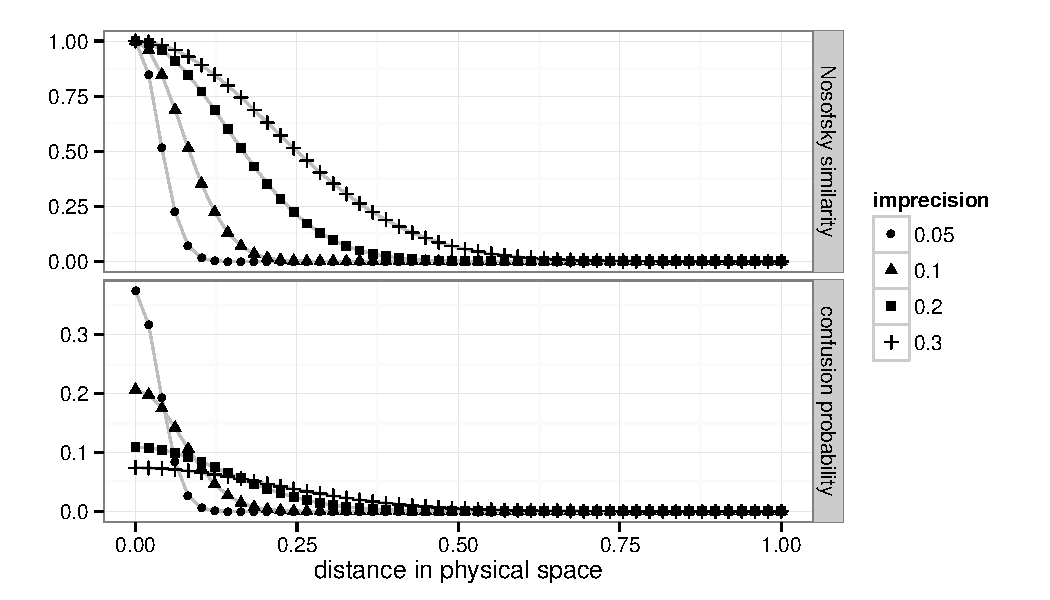
\includegraphics[width=\textwidth]{plots/NosofskySim.pdf}

  \caption{Examples for Nosofsky-similarity (non-normalized) and
    derived probability of state confusion (normalized) for
    $\card{\States} = 50$ and different
    values of $\impairment$.}
  \label{fig:NosofskySim}
\end{figure}





We further assume that the probability of confusing any two states
$\mystate{i}$ and $\mystate{j}$ is proportional to their perceived
similarity and therefore obtained by normalization:
\begin{align*}
  C_{ij} = \frac{\similarity(\mystate{i}, \mystate{j} \myts ; \myts
  \impairment)} {\sum_j \similarity(\mystate{i}, \mystate{j} \myts ; \myts
  \impairment)} \,.
\end{align*}
Confusion of states is then also a function of imprecision parameter
$\impairment$ (see Figure~\ref{fig:NosofskySim}, bottom part). For $\impairment
= 0$ the confusion matrix has $C_{ii} = 1$; for $\impairment > 0$ $C$ is
positive, i.e., $C_{ij} >0$ for all $i$ and $j$; for $\impairment
\rightarrow \infty$ we find $C_{ij} = \nicefrac{1}{\card{\States}}$ for all
$i$ and $j$.

Difusion of behavior under confusion of states was defined in
Equation~(\ref{eq:confusion-function}), repeated here:
\begin{align*}
  \Diff_C(\Sstrat) & = C \Sstrat &    \Diff_C(\Rstrat) & = \Rstrat C\,.
\end{align*}
If states are confused on average with a probability proportional to
their similarity, the effect on noise-perturbed behavior is that
behavioral dispositions gradually diffuse along a gradient of
similarity of states as well. Consequently, iterated diffusion leads
to a smoothing out and an eventual equalization of behavioral
strategies, for both the sender and the
receiver. Figure~\ref{fig:confusion-SenRec} shows an arbitrary sender
and receiver strategy after one or several rounds of iterated
application of diffusion, for different values of perceptual
imprecision $\impairment$.

The example in Figure~\ref{fig:confusion-SenRec} suggests that
iterated diffusion leads to sender and receiver behavior that is the
same at all choice points. This holds in general. After $n$ steps of
diffusion an initial sender strategy $\Sstrat$ will be $C^n \Sstrat$,
and an initial receiver strategy $\Rstrat$ will be $\Rstrat C^n$. If
we assume that $\impairment > 0$, $C$ is a positive row-stochastic
matrix (each state could in principle be confused as any other state,
albeit with possibly a very low probability). It then follows from the
Perron-Frobenius theorem that the limit $C^\infty = \lim_{n
  \rightarrow \infty} C^n$ exists (it is the Perron-projection) and
all of its rows are identical. That is why, in the limit of iterated
diffusion, $C^\infty S$ has identical rows (messages are sent with the
same probability in each state), and $R C^\infty$ likewise has
identical rows (every message is interpreted equally). All of this is
in line with the intuition that diffusion of behavior under confusion
of states iteratively equalizes behavior for similar states; if all
states can be confused for one another in principle, behavior smoothes
out entirely in the limit.

\begin{figure}
  \centering

  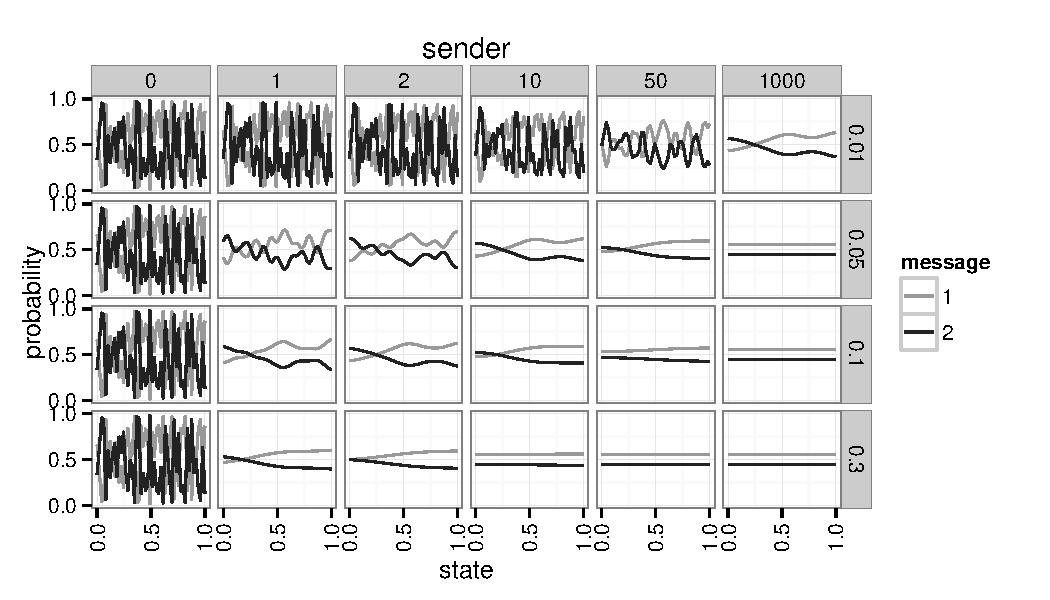
\includegraphics[width=\textwidth]{plots/confusion_sender.pdf}
  
  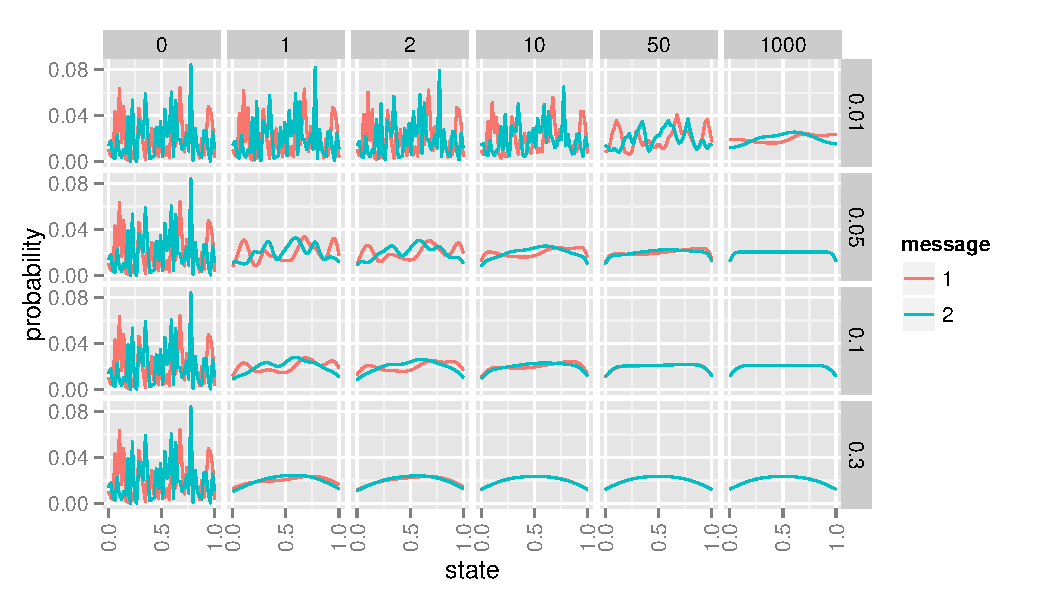
\includegraphics[width=\textwidth]{plots/confusion_receiver.pdf}

  \caption{Iterated diffusion for one arbitrary sender (top) and one
    receiver strategy (bottom), for a game with 50 states and 2
    messages. Each row corresponds to a different confusion level
    $\impairment$, each colum to a different number of applications of
    iterated diffusion.}
  \label{fig:confusion-SenRec}
\end{figure}

\subsection{Exploring the replicator diffusion dynamics}
\label{sec:simulations}

Now that we understand better what diffusion does, let us look at how
diffusion interacts with optimization of behavior, as described by the
replicator dynamics. The main question we should address is whether
diffusion and fitness-based replication reasonably interact, and if
so, whether the inclusion of diffusion has any noteworthy effects on
the evolving meaning of signals. Clearly, if $\impairment = 0$, the
\rdd reduces to the \rd. If $\impairment \rightarrow \infty$, the
diffusion component takes over and the \rdd reduces to the trivial
iterated diffusion that we looked at in the previous section. We will
show presently that for reasonable in-between levels of imprecision
$\impairment$, the \rdd leads to communicatively successful, yet vague
signal meaning. Suitable levels of imprecision can have further
accelerating and unifying effects on meaning evolution.

\subsubsection{Experimental set-up}

To explore the \rdd, we looked at numerical simulations in sim-max
games with two signals whose states were evenly spaced elements of the
unit interval that always included 0 and 1. We assumed that priors
were flat: $\Pr(\state) = \Pr(\state')$ for all $\state, \state'$. As
for utility functions, we implemented another Nosofsky-style function:
\begin{align}
  \label{eq:NosofskyUtil}
  \util(\mystate{i}, \mystate{j} \myts ; \myts \toler) =
      \begin{cases}
    1 & \textrm{if } \impairment = 0 \textrm{ and } \mystate{i} = \mystate{j} \\
    0 & \textrm{if } \impairment = 0 \textrm{ and } \mystate{i} \neq \mystate{j} \\
 \expo \left ( -  \frac{\card{\mystate{i} - \mystate{j}}^s}{ \toler^2} \right ) \,,& \textrm{otherwise} \\
    \end{cases}
\end{align}
The tolerance parameter $\toler > 0$ models the amount of tolerable
pragmatic slack or communicative imprecision. This choice of utility
function is governed partly by convenience in parallel to the
similarity function, but also because it has, as we believe, the right
general properties for a communicative payoff function. Unlike
utilities that are, say, linearly or quadratically decreasing in
physical distance \citep[as used
by][]{JagerMetzger2011:Voronoi-Languag,FrankeJager2010:Vagueness-Signa},
utilities that are exponentially decreasing in negative quadratic
distance can model situations where a small amount of imprecision in
communication is tolerable, whereas similarly small differences in
intolerably far away interpretations matter very little, with a smooth
transition between these regimes
\citep[c.f.][]{OConnor2013:The-Evolution-o}.

\begin{figure}
  \centering

  \begin{subfigure}[]{0.45\textwidth}
    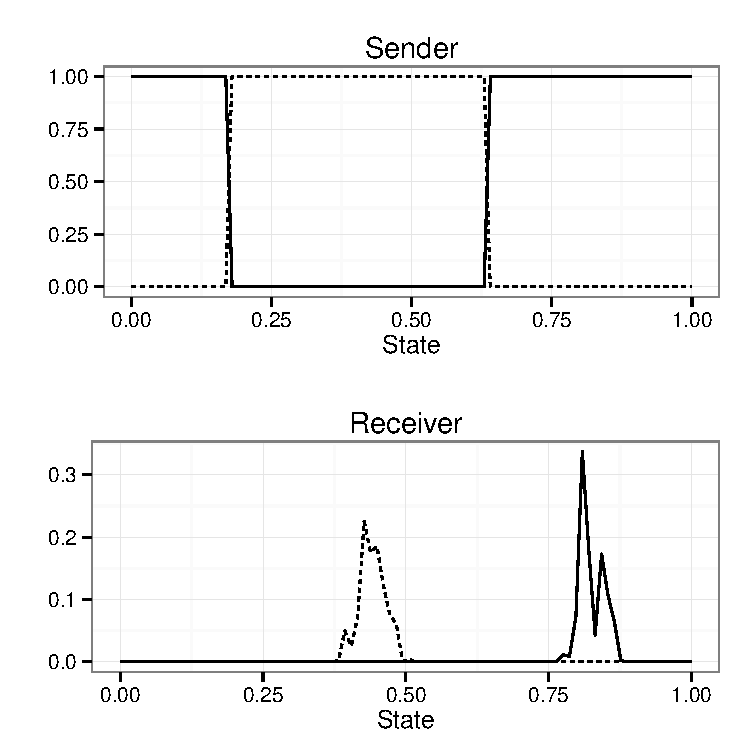
\includegraphics[width=\textwidth]{plots/strat_example_NS-90_tol-01_imp0_ind3098.pdf}
    \caption{$\ns = 90$, $\toler = 0.1$, $\impairment = 0$}
    \label{fig:example_stratsA}
  \end{subfigure}
  \hfill
  \begin{subfigure}[]{0.45\textwidth}
    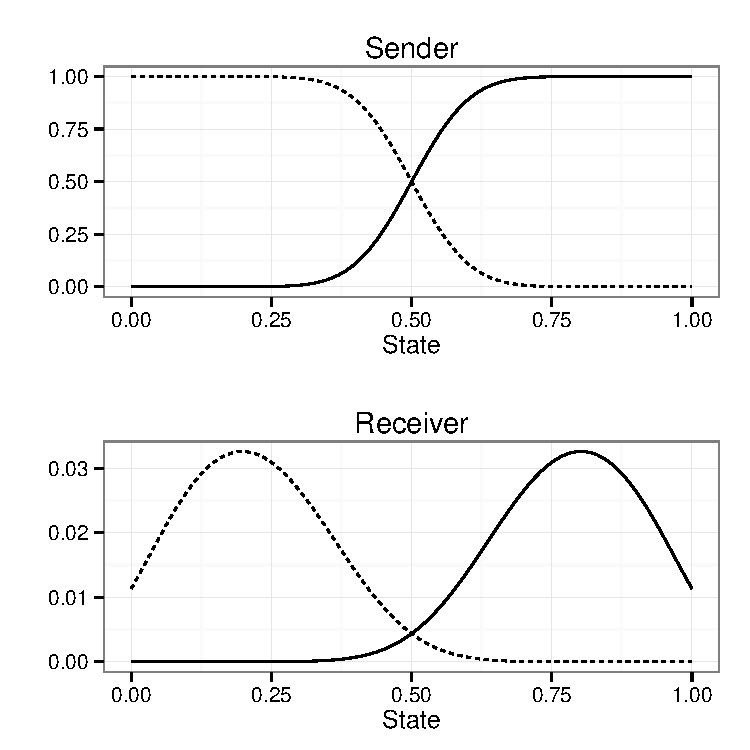
\includegraphics[width=\textwidth]{plots/strat_example_NS-90_tol-01_imp01_ind3452.pdf}
    \caption{$\ns = 90$, $\toler = 0.1$, $\impairment = 0.1$}
    \label{fig:example_stratsB}
  \end{subfigure}

  % \begin{subfigure}[]{0.45\textwidth}
  %   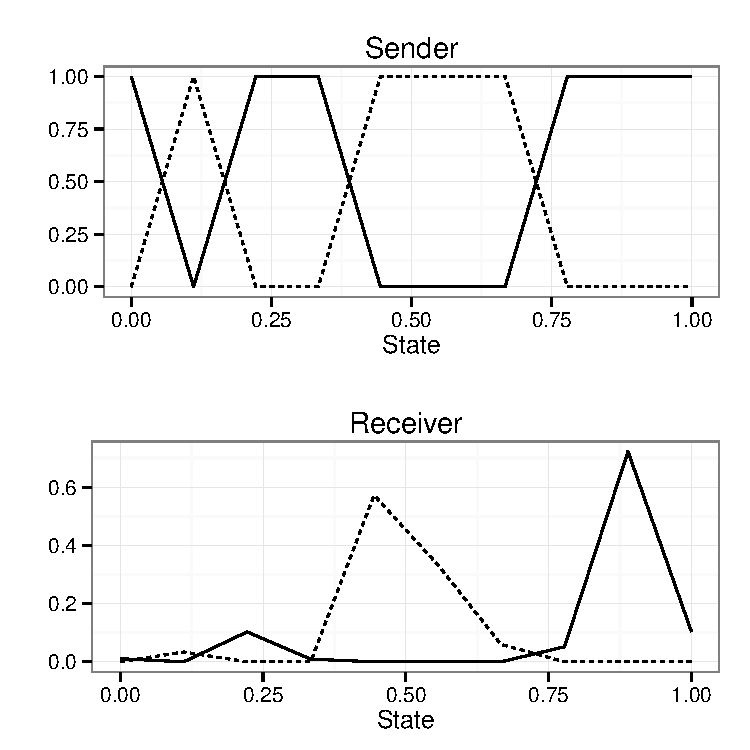
\includegraphics[width=\textwidth]{plots/strat_example_NS-10_tol-005_imp0_ind1001.pdf}
  %   \caption{$\ns = 10$, $\toler = 0.1$, $\impairment = 0$}
  %   \label{fig:example_stratsC}
  % \end{subfigure}
  % \hfill
  % \begin{subfigure}[]{0.45\textwidth}
  %   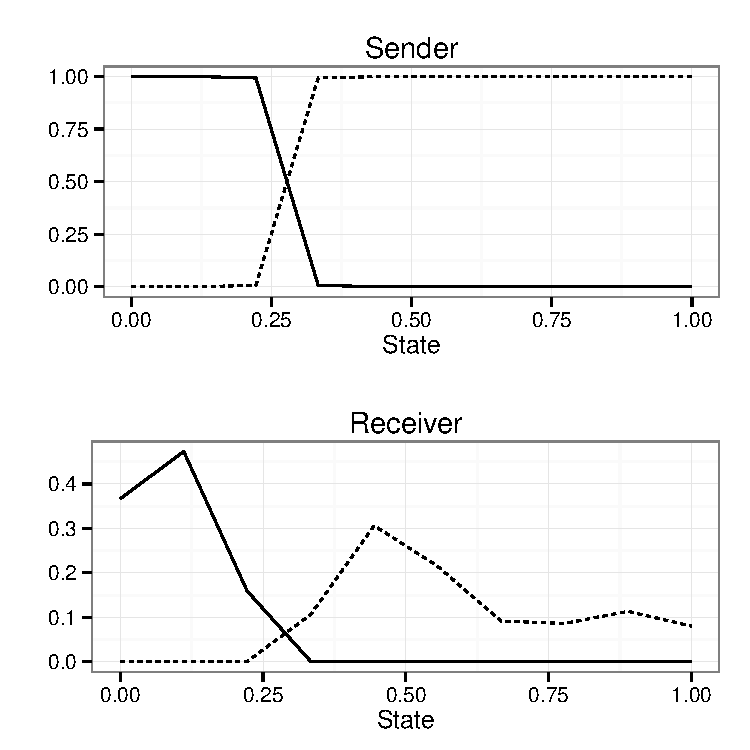
\includegraphics[width=\textwidth]{plots/strat_example_NS-10_tol-005_imp005_ind1201.pdf}
  %   \caption{$\ns = 10$, $\toler = 0.1$, $\impairment = 0.05$}
  %   \label{fig:example_stratsD}
  % \end{subfigure}


  \caption{Example strategies under \rdd at stopping time of our simulations.}
  \label{fig:example_strats}
\end{figure}

We ran 50 trials of the \rdd, starting with randomly sampled sender
and receiver strategies, for each triplet of independent parameter
values: $\ns = \card{T} \in \set{6, 10, 50, 90}$, $\impairment \in
\set{0, 0.05, 0.1, 0.2, 0.3}$, $\toler \in \set{0.05, 0.1, 0.2,
  0.3}$. Each trial ran for a maximum of 200 update steps of the
\rdd. This may not be enough to guarantee convergence to the eventual
attracting state, but we were interested especially in whether the
dynamics could lead to reasonable outcomes in reasonable time. A trial
was considered converged and stopped before the maximum of 200 rounds
if the total amount of change between strategies before and after the
current \rdd step was smaller than 0.001, i.e., if:
\begin{align*}
  \sum_{\state \in \States} \sum_{\messg \in \Messgs} \left|
    \rdd(\Sstrat)(\state,\messg) - \Sstrat(\state,\messg) \right| <
  0.001\,, & \text{\ \ and} \\
  \sum_{\messg \in \Messgs} \sum_{\state \in \States} \left|
    \rdd(\Rstrat)(\messg,\state) - \Rstrat(\messg,\state) \right| <
  0.001 & \,.
\end{align*}

Representative examples for resulting strategy pairs at stopping time
are given in
Figure~\ref{fig:example_strats}. Figure~\ref{fig:example_stratsA}
shows a strategy pair at stopping time with 90 states, tolerance
$\toler = 0.1$ and imprecision $\impairment = 0$. The latter means
that the trial was effectively a plain application of the
\rd. Noteworthily, the given sender strategy approximates a pure
sender strategy that crisply partitions the state space into
non-convex sets. The irregular shape of the receiver strategy shows
clearly that the pictured strategy pair has not yet reached a
dynamically stable state under the \rd. Indeed, the trial did not
converge in our technical sense, but was stopped after 200 rounds of
iterated \rdd. In contrast, the outcome of a trial with identical
parameters, except that imprecision was $\impairment = 0.1$, is shown
in Figure~\ref{fig:example_stratsB} had converged (in our technical
sense) after 99 rounds of iterated \rdd. The sender strategy shows a
smooth blending from one ``category'' to the other, and the receiver's
interpretations are rather extended curves, peaking at a central point
in the relevant ``categories''. What these examples show is that (i),
contrary to the limiting results of
\citet{Jager2007:The-Evolution-o,JagerMetzger2011:Voronoi-Languag},
(speaker) strategies can approach non-convex pure strategies and that
(ii) inclusion of imprecision can lead to seemingly well-behaved, yet
vague strategies in the sense that we are after.

\subsubsection{Dependent measures}
 
To explore further what happened in all of our 50 trials for each
parameter triple, we defined a small number of metrics that aim to
capture numerically how vague, communicatively efficient and generally
well-structured the resulting strategy pairs were. Entropy and
informativity capture (slightly different aspects of) the amount of
systematicity or regularity in a language. Voronoiness and convexity
are, respectively, gradient and categorical measures for the coherence
of linguistically formed categories. Expected utility measures the
communicative efficiency of evolved strategy pairs. 

\paragraph{Entropy.} This classic information-theoretic metric
captures the amount of uncertainty in a signaling strategy. Roughly
put, entropy of a strategy captures inverse distance from a pure
strategy. The most natural way to define it is in terms of mixed
strategies rather than behavioral strategies.  Let us recall that
mixed sender (receiver) strategies are functions $\Smixed \in
\Delta(\Messgs^\States)$ ($\Rmixed \in (\Acts^\Messgs)$).  We can
define the entropy of a sender and receiver strategy as
\begin{align*}
  E(\Smixed) & = \sum_{\Spure \in \Messgs^\States} \Smixed(\Spure) \cdot
  \log(\Smixed(\Spure)) & 
  E(\Rmixed) & = \sum_{\Rpure \in \Acts^\Messgs} \Rmixed(\Rpure) \cdot \log(\Rmixed(\Rpure)) \,.
\end{align*} 
These measures are computationally expensive to calculate, since the
size of the domain over which the sum is computed grows exponentially
with the number of choice points.  Therefore, we
converted\footnote{See Appendix~\ref{sec:proofs}.}\todo{include
  this!?} the above definitions into equivalent metrics defined in
terms of behavioral strategies.  These are as follows:
\begin{align*}
  E(\Sstrat) = -\sum_{\state \in \States} \sum_{\messg \in \Messgs}
  \Sstrat(\messg \probbar \state) \cdot \log(\Sstrat(\messg \probbar
  \state)) 
\end{align*} 
\begin{align*}
  E(\Rstrat) = -\sum_{\messg \in \Messgs} \sum_{\act \in \Acts}
  \Rstrat(\act \probbar \messg) \cdot \log(\Rstrat(\act \probbar
  \messg)) \,. 
\end{align*}
Values obtained by these definitions are lower bounded by $0$ and
upper bounded by, respectively, $\log(|\Messgs^\States|) = |\States|
\cdot \log(|\Messgs|)$ and $\log(|\Acts^\Messgs|) = |\Messgs| \cdot
\log(|\Acts|)$. We work with normalized values. 

The speaker strategies in Figures~\ref{fig:example_stratsA} and
\ref{fig:example_stratsB} have entropy $1.19e^{-5}$ and $0.21$,
respectively. The receiver strategies have respective entropies $0.43$
and $0.84$. In general, we expect that vague languages will have
higher entropy than crisp ones and that increasing imprecision will
also increase entropy, all else being equal.



\paragraph{Informativity.} The quantity of information in a signal is
an old notion that also goes back to the start of information theory.
\citet[ch.~3]{Skyrms2010:Signals} discusses its use in the context of
signaling games. Intuitively speaking, informativity in Skyrms' sense
measures how revealing the sender's signal use is about which state is
actual. It therefore measures, in our given set-up with flat priors, a
sense of well-behavedness or regularity of a sender strategy.

The main idea behind Skyrm's notion is that we can quantify the amount
of information about a state $\state$ in a message $\messg$ via the
relation between the probability of the state given the message
$\Pr(\state \,|\, \messg)$ and the unconditional probability of the
state $\Pr(\state)$.  Following Bayes' theorem, we can express
$\Pr(\state \,|\, \messg)$ as $\frac{\Pr(\state) \cdot \Pr(\messg
  \,|\, \state)}{\Pr(\messg)}$.  We then have $\Pr(\messg \,|\,
\state) = \Sstrat(\state,\messg)$ and $\Pr(\messg) =
\sum_{\state^\prime \in \States} \Pr(\state^\prime) \cdot
\Sstrat(\state^\prime,\messg)$.  Finally, we equate sender
infomativity with the average overall information about states in each
signal.  Following \citet[p.~36]{Skyrms2010:Signals}, and the
considerations above, the informativity about states conveyed by a
sender strategy is:
\begin{align*}
  I(\Sstrat) = \frac{1}{|\Messgs|} \sum_{\messg \in \Messgs}
  \sum_{\state \in \States} \frac{\Pr(\state) \cdot
    \Sstrat(\state,\messg)}{\sum_{\state^\prime \in \States}
    \Pr(\state^\prime) \cdot \Sstrat(\state^\prime,\messg)} \cdot \log
  \left(\frac{\Sstrat(\state,\messg)}{\sum_{\state^\prime \in \States}
      \Pr(\state^\prime) \cdot \Sstrat(\state^\prime,\messg)} \right)
  \,. 
\end{align*}
This measure is bounded between $0$ and $1$. The speaker strategies in
Figures~\ref{fig:example_stratsA} and \ref{fig:example_stratsB} have
informativity $0.69$ and $0.54$, respectively. In general, we expect
that vague languages will have lower informativity than crisp
ones and that increasing imprecision will decrease informativity. 

\citet[p.~39]{Skyrms2010:Signals} also offers a notion of
informativity about the acts performed by the receiver, but it turns
out that this is perfectly correlated with information about the
states in the results of our simulations. We therefore only look at
informativity about states. 

% Conversely, we can quantify the amount of information about an act in a message.
% We equate receiver informativity with the average overall information about acts in each signal.
% Based on Skyrms' definition~\citet[p.~39]{Skyrms2010:Signals}, we define receiver informativity as follows:
% \begin{align*}
%   I(\Sstrat,\Rstrat) = \frac{1}{|\Messgs|} \sum_{\messg \in \Messgs} \sum_{\act \in \Acts} \Rstrat(\messg,\act) \cdot \log \left(\frac{\Rstrat(\messg,\act)}{\sum_{\state \in \States} \Pr(\state) \cdot \sum_{\messg^\prime \in \Messgs} \Sstrat(\state,\messg^\prime) \cdot \Rstrat(\messg^\prime,\act)} \right) \,.
% \end{align*}

\paragraph{Voronoiness.}
This metric aims to quantify how close a strategy is to being a part
of a Voronoi tessallation of the state space. Bearing in mind that
this metric is specifically geared towards the sim-max games in our
set-up, we define Voronoiness as follows. Let $\pi(\Rstrat, \messg) =
\argmax_{\state \in \States}\Rstrat(\messg,\state)$ be the prototype
of a message $\messg \in \Messgs$, then
\begin{multline*}
  V(\Sstrat, \Rstrat) = \sum_{\state \in \States} \sum_{\messg_1 \in
    \Messgs} \sum_{\messg_2 \in \Messgs} \textrm{if } s(\state,
  \pi(\Rstrat, \messg_1)) > s(\state, \pi(\Rstrat, \messg_2)) \bicond
  \Sstrat(\state, \messg_1) > \Sstrat(\state, \messg_2) \textrm{ then
  } 1 \textrm{ else } 0 
\end{multline*}
is the Voronoiness of the sender strategy $\Sstrat$ given the receiver
strategy $\Rstrat$ and
\begin{align*}
  V(\Rstrat) = \sum_{\messg \in \Messgs} \sum_{\state_1 \in \States}
  \sum_{\state_2 \in \States} \textrm{if } s(\state_1, \pi(\Rstrat,
  \messg)) > s(\state_2, \pi(\Rstrat, \messg)) \bicond \Rstrat(\messg,
  \state_1) > \Rstrat(\messg, \state_2) \textrm{ then } 1 \textrm{
    else } 0
\end{align*}
is the Voronoiness of the receiver strategy $\Rstrat$.  The metrics
are lower bounded by $0$ and upper bounded by, respectively,
$|\States| \times |\Messgs|^2$ and $|\Messgs| \times |\States|^2$,
thus we can normalize them by dividing by these values.

Despite being vague, a language can have maximal Voronoiness according
to this gradient measure. For instance, the sender strategies in
Figures~\ref{fig:example_stratsA} and \ref{fig:example_stratsB} have
Voronoiness $0.91$ and $1$, respectively. The receiver strategies have
Voronoiness $0.78$ and $1$, respectively. We do not \emph{prima facie}
expect a conceptual connection between vagueness and Voronoiness, and
so do not predict a clear effect of imprecision on Voronoiness either.

\paragraph{Convexity.} At least for speaker strategies, which converge
faster, it also makes sense to define a categorical measure of
convexity, that compensates for potential vagueness. To determine
whether a sender strategy $\Sstrat$ was convex despite possibly being
vague, we looked at the derived pure strategy $\Spure$ for which
$\Spure(\state) = \messg$ only if $\messg =
\argmax_{\messg' \in \Messgs} \Sstrat(\state,\messg')$. If that $\Spure$
was convex, we also counted $\Sstrat$ as convex. The sender strategy
in Figure~\ref{fig:example_stratsA} is not convex, while the one in
Figure~\ref{fig:example_stratsB} is. Again, we do not expect a
conceptual relation between vagueness and imprecision, on the one
hand, and convexity on the other.

\paragraph{Expected utility.} We also recorded the expected utility of
a strategy pair:
\begin{align*}
  \EU(\Sstrat,\Rstrat \myts ; \myts \toler) = \sum_{\state \in
    \States} \sum_{\messg \in \Messgs} \sum_{\state' \in \States}
  \Pr(\state) \cdot \Sstrat(\state, \messg) \cdot \Rstrat(\messg,
  \state') \cdot \Util(\state,\state' \myts ; \myts \toler)\,.
\end{align*}
To make direct comparisons across different parameter settings, we
normalized expected utility by the maximal amount of expected utility
obtainable in the relevant game. 

The strategy pair in Figure~\ref{fig:example_stratsA} has a normalized
expected utility of $0.992$, the pair in
Figure~\ref{fig:example_stratsB} has $0.901$. Generally, vagueness and
imprecision can be expected to decrease expected utility
\citep{Lipman2009:Why-is-Language}. The crucial question is whether
communicative success drops unacceptably fast with moderate levels of
vagueness and imprecision.

\subsubsection{Results}

\begin{figure}
  \centering
  
  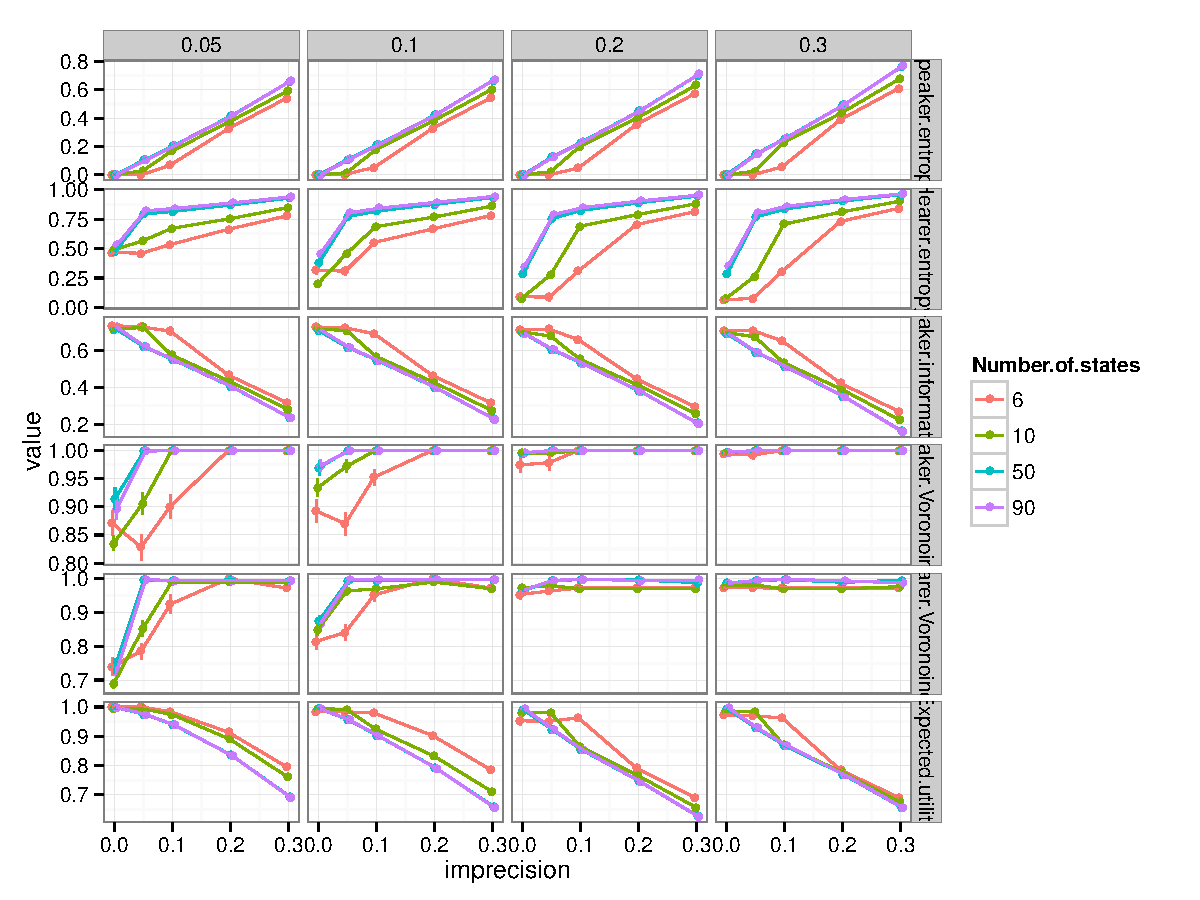
\includegraphics[width=\textwidth]{plots/MeanMetrics.pdf}

  \caption{Means of recorded metrics for each triple of independent variables.}
  \label{fig:MeanMetrics}
\end{figure}

Figure~\ref{fig:MeanMetrics} shows the means of the recorded metrics,
together with their estimated 95\% confidence intervals, for each
triple of independent variables. Most trends are quite clear, and not
unexpected. Entropy of sender and receiver strategies are increasing
in imprecision. Entropy of speaker strategies seems independent of
tolerance levels and the number of states, while there seems to be an
effect of both parameters on the entropy of the hearer
strategy. Speaker informativity and expected utility are decreasing
under growing imprecision. There seem to be mild effects of the number
of states in the game, but hardly any in terms of pragmatic
tolerance. What was not expected \emph{a priori} was that Voronoiness
of both sender and receiver strategies appear to be non-decreasing
under increasing impairment and peaking at the maximal value. The only
exception is the 6 states games and the transition from $\impairment =
0$ to $\impairment = 0.05$. Expected utility of evolved languages
mostly decreases in increasing imprecision, with the sole exception of
a rise for $\toler = 0.2$ and $ns = 6$ at $\impairment = 0.1$. Still,
normalized expected utility of evolved strategy pairs under mild
values of imprecision are not necessarily much worse than their
respective perfect precision \rd-analogues. This is especially so for
lower numbers of states (which increase the chance of non-convergence
and non-convexity; see Figure~\ref{fig:CategoricalMeasures} and the
discussion below).




Taken together, these findings suggest the following effect of
imprecise perception and diffusion of behavior. Mild forms of
perceptual imprecision lead to slightly less communicative efficiency
in the evolving strategy pairs, more vagueness and more regular,
well-behaved languages. This impression is also supported by the
proportion of converged and convex trials, pictured in
Figure~\ref{fig:CategoricalMeasures}. Non-converged and non-convex
speaker strategies showed for several values of parameters in the
absence of impairment. Increasing impairment always assured
convergence and convexity: perceptual imprecision speeds up
convergence to a convex and regular language.

\begin{figure}
  \centering
  
  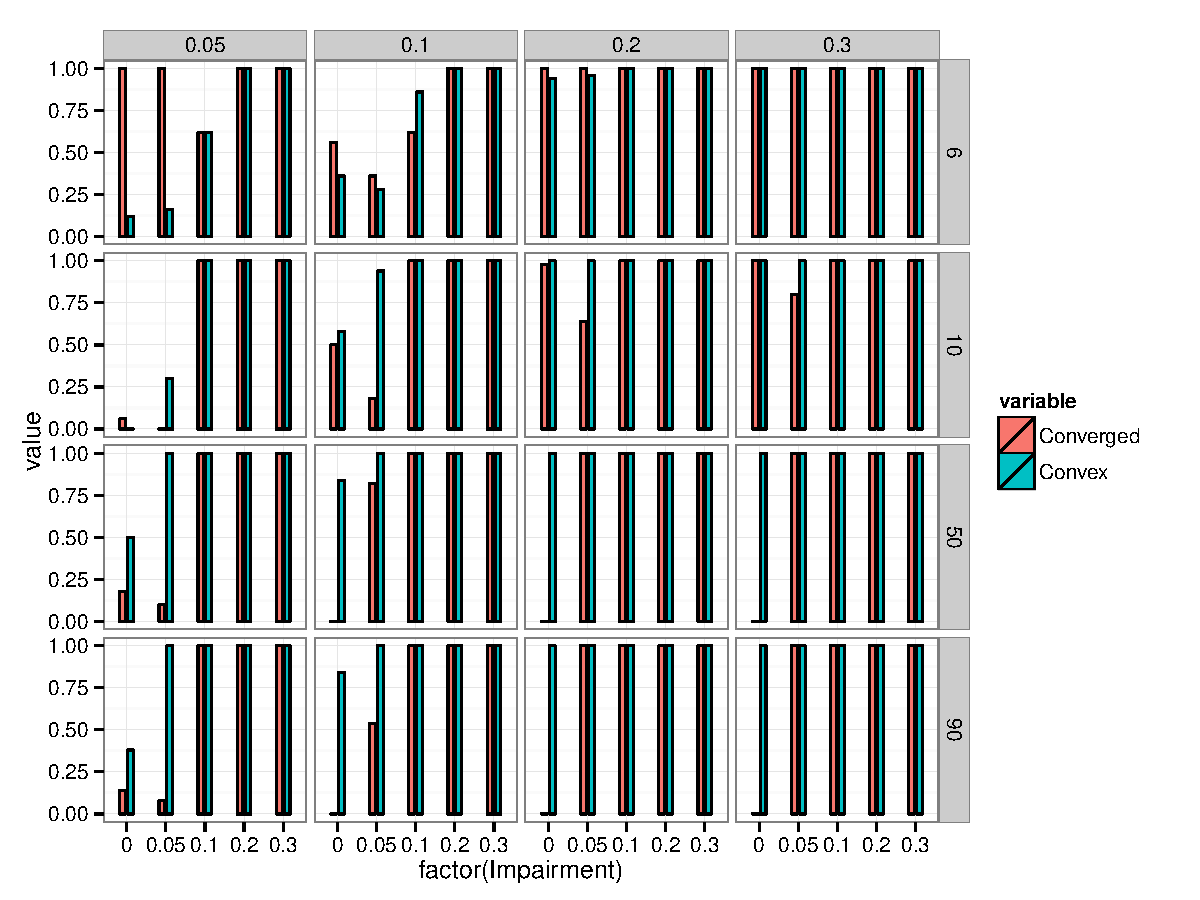
\includegraphics[width=\textwidth]{plots/CategoricalMeasures.pdf}

  \caption{Proportion of converged and convex trials.}
  \label{fig:CategoricalMeasures}
\end{figure}

Diffusion also has another interesting regularizing effect on the
evolution of signaling. If we look at the confidence intervals in
Figure~\ref{fig:MeanMetrics}, we see that there is very little
variation in the recorded metrics for evolved strategies, at least for
higher values of impairment. On closer inspection, it turns out that
variability in low-impairment conditions is not only due to
non-convergence and/or associated
non-convexity. Figure~\ref{fig:MoreExample_strats} gives two more
examples of strategy pairs at stopping time. Both are obtained for the
same triple of parameters, both converged and are convex. However,
they are not equally efficient. In fact, the pair in
Figure~\ref{fig:example_stratsC} has a normalized expected utility of
$0.99$ while the one in Figure~\ref{fig:example_stratsD} only has
$0.89$.


\begin{figure}
  \centering

  \begin{subfigure}[]{0.45\textwidth}
    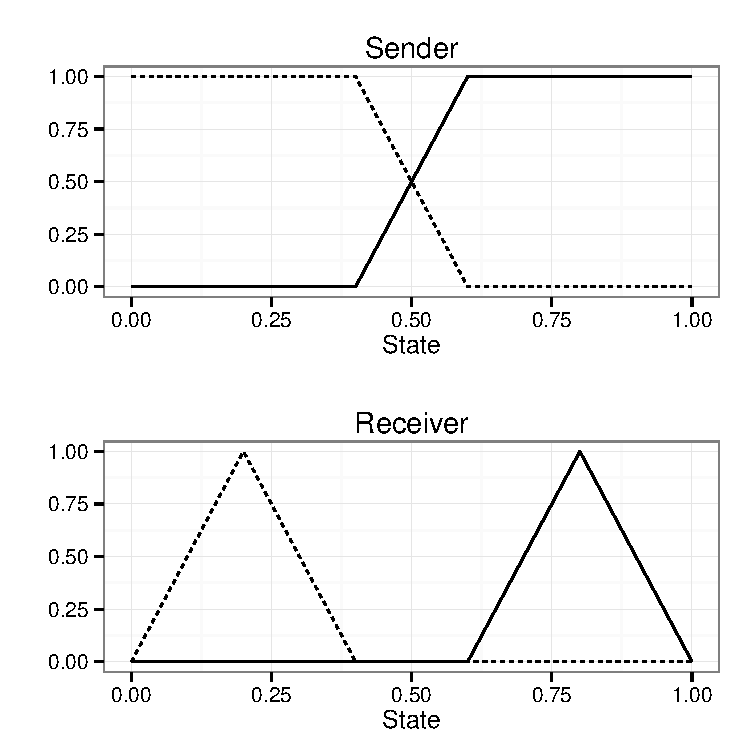
\includegraphics[width=\textwidth]{plots/strat_example_NS-6_tol-03_imp005_ind41.pdf}
    \caption{$\ns = 6$, $\toler = 0.2$, $\impairment = 0$}
    \label{fig:example_stratsC}
  \end{subfigure}
  \hfill
  \begin{subfigure}[]{0.45\textwidth}
    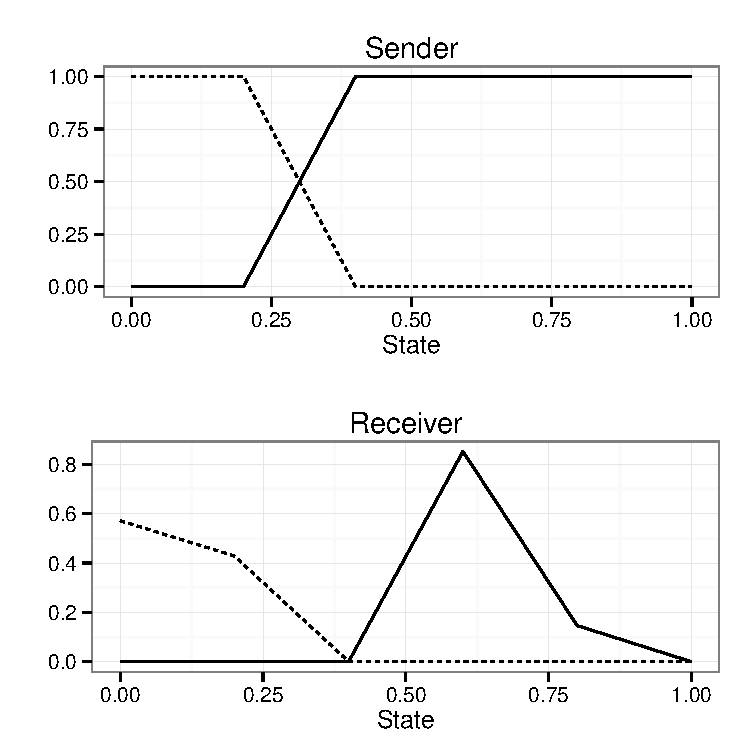
\includegraphics[width=\textwidth]{plots/strat_example_NS-6_tol-03_imp005_ind23.pdf}
    \caption{$\ns = 6$, $\toler = 0.2$, $\impairment = 0$}
    \label{fig:example_stratsD}
  \end{subfigure}

  \caption{More example strategies under \rdd at stopping time of our simulations.}
  \label{fig:MoreExample_strats}
\end{figure}

Interestingly, this type of variability in evolutionary outcomes is
also weeded out by mild increases in impairment. To see this, we
calculated the average distance between evolved sender strategies
within each group of trials that had identical independent
parameter values. We determined the distance between sender strategies
$\Sstrat$ and $\Sstrat'$ as the average Hellinger distance between
probability distributions $\Sstrat(\state)$ and $\Sstrat'(\state)$
over messages at each choice point $\state$:
\begin{align*}
  \text{HD}(\Sstrat,\Sstrat') & = \frac{1}{{\card{\States} \cdot
     \sqrt{2}}} \cdot  \sum_{\state \in \States} 
 \sqrt{\sum_{\messg \in  \Messgs}
         \left ( \sqrt{\Sstrat(\state,\messg)} -
         \sqrt{\Sstrat'(\state,\messg)} \right )^2 }\,.
\end{align*}
To compensate for the arbitrariness of message use, we set the
distance between strategies $\Sstrat$ and $\Sstrat'$ to be the maximum
of $\text{HD}(\Sstrat,\Sstrat')$ and $\text{HD}(\Sstrat^*,\Sstrat')$
where $\Sstrat^*$ is $\Sstrat$ with reversed message indices. The
average distances between sender strategies in this sense is plotted
in Figure~\ref{fig:AverageEUinGroups}. This clearly shows that with
increasing imprecision, the sender strategies evolving under \rdd were
exactly alike, modulo which message was used for which part of the
unit interval. In other words, perceptual imprecision clearly unifies
evolutionary outcomes, and in fact guarantees sender strategies that
are not only convex, but also maximally efficient in that they induce
a vague category split exactly in the middle of the unit interval.

\begin{figure}
  \centering

    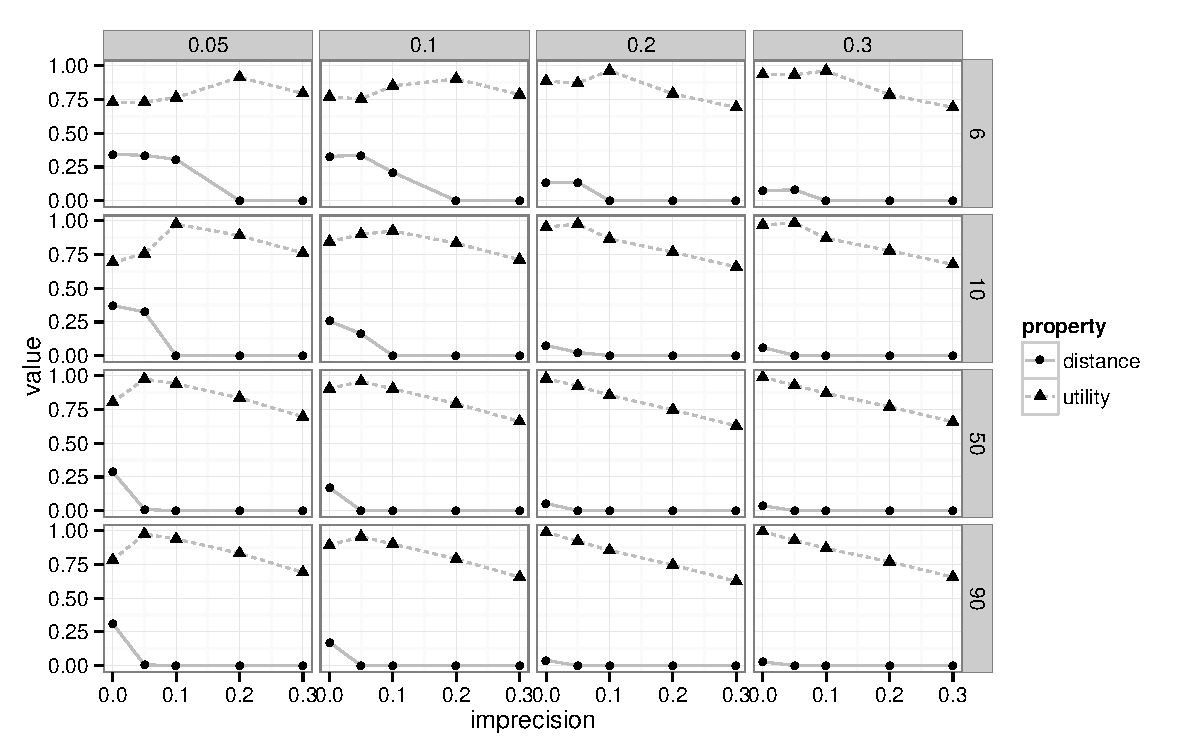
\includegraphics[width=\textwidth]{plots/WithinGroupMeasures.pdf}

    \caption{Mean group measures as defined in the main text. For each
      group, i.e., triplet of independent variables, the plot shows
      (i) average normalized expected utility when playing against an
      arbitrary other language from the group, (ii) the mean distance
      between evolved sender strategies in the group.}
  \label{fig:AverageEUinGroups}
\end{figure}

This unifying property of perceptual imprecision could be considered
an evolutionary beneficial side-effect. When we look at the normalized
average expected utility that each evolved language (i.e., pair of
sender and receiver strategy at stopping time) scored when playing
against an arbitrary other language of the same group in
Figure~\ref{fig:MoreExample_strats}, we see that higher imprecision
can lead to higher such average expected utility. What this means is
that, imprecision might decrease the communicative efficiency of
individual languages, it increases the conceptual coherence and
communicative success between independently evolving strategies. It is
almost as if mere confusability of states imposes a regularity
constraint on evolving linguistic meanings.

%%% Local Variables: 
%%% mode: latex
%%% TeX-master: "paper"
%%% TeX-PDF-mode: t
%%% End:



